%% LyX 2.2.4 created this file.  For more info, see http://www.lyx.org/.
%% Do not edit unless you really know what you are doing.
\documentclass[english]{article}
\usepackage{lmodern}
\usepackage[T1]{fontenc}
\usepackage[latin9]{inputenc}
\usepackage{geometry}
\geometry{verbose,tmargin=3cm,bmargin=3cm,lmargin=2.5cm,rmargin=2.5cm}
\usepackage{textcomp}
\usepackage{graphicx}
%\usepackage{mcode}

\renewcommand\thesection{\alph{section}}

\makeatletter

%%%%%%%%%%%%%%%%%%%%%%%%%%%%%% LyX specific LaTeX commands.
%% Because html converters don't know tabularnewline
\providecommand{\tabularnewline}{\\}

\makeatother

\usepackage{babel}

\usepackage{pdfpages}



\begin{document}

\includepdf{cover1.pdf}
\title{4F13: Probabilistic Machine Learning\\
 Gaussian Processes}

\author{Candidate number: 5673D \\
		Words count: approximetly 1150
	}

\maketitle

\section{GP with a squared exponential SE covariance function \label{a}}
	We want to fit the 1-D data loaded from \texttt{cw1a.mat} using a 0-mean Gaussian Process with Squared Exponential (SE) covariance function. Assuming our observations have WGN with variance $\sigma_n^2$, we can compute the covariance between targets as:
	
\begin{equation}
	k(x_i, x_j) = \sigma^2 \exp\left( - \frac{(x_i - x_j)^2}{2 l^2} \right) + \delta_{ij} \sigma_{n}^2
\end{equation}
where $\sigma^2 > 0 $ is the signal variance, $l > 0$ is the length scale and $\delta_{ij}$ is Kronecker delta. 
The hyper-parameters of this model are $\theta = (l, \sigma, \sigma_n)$. The length scale ($l$) determines the smoothness of the function. A low-valued $l$ means that our data is weakly correlated (equivalent of a low signal to noise ratio) and our model will have troubles extrapolating further away from out data points and will tend to fluctuate more quickly. A high-valued $l$ means a strong correlation between the points, therefore better approximations for point further away from our data.

The optimal values for our hyper-parameters are calculated by minimizing the negative marginal log-likelihood $-\log(p(y|x,\theta))$ wrt. the hyper-parameters $\theta$ using the code below.     

\begin{verbatim}
	S = load('cw1a.mat')
	hyp = struct('mean', [], 'cov', [0 0], 'lik', -1);
	covfunc = @covSEiso; %set the Covariance fuction as SE	
	meanfunc = [];
	likfunc = @likGauss;
	hyp.cov = [-1, 0]; hyp.lik = 1; %initialise hyperparameters
	%minimise negative log marginal likelyhood
	hyp2 = minimize(hyp, @gp, -100, @infGaussLik, meanfunc, covfunc, likfunc, x, y);
	%set targets
	xs = linspace(-3, 3, 100)'; 
	%train GP
	[mu s2] = gp(hyp2, @infGaussLik, meanfunc, covfunc, likfunc, x, y, xs);
\end{verbatim}
	
We get the following minimum $log(p(y|x,\theta) = -11.9$, corresponding to $\mathbf{\theta} =  (0.128, 0.897, 0.118) ) $. The predictions are shown in Figure 1, on the left, in orange and the $95\%$ error bars in grey. The small length scale effect can be clearly seen. The error bars are tight around the data and are larger in regions with few data points. In the regions with many data points the lower bound of the error bars is $2\sigma_n$, while in the other regions increases to $2\sigma$. This makes the model good at interpolation and while not being efficient for extrapolation. Moreover this optimization prevents the model from over-reducing the values for length scale and noise variance, thus avoiding overfitting.   

	\begin{figure}[h]
		\begin{centering}
			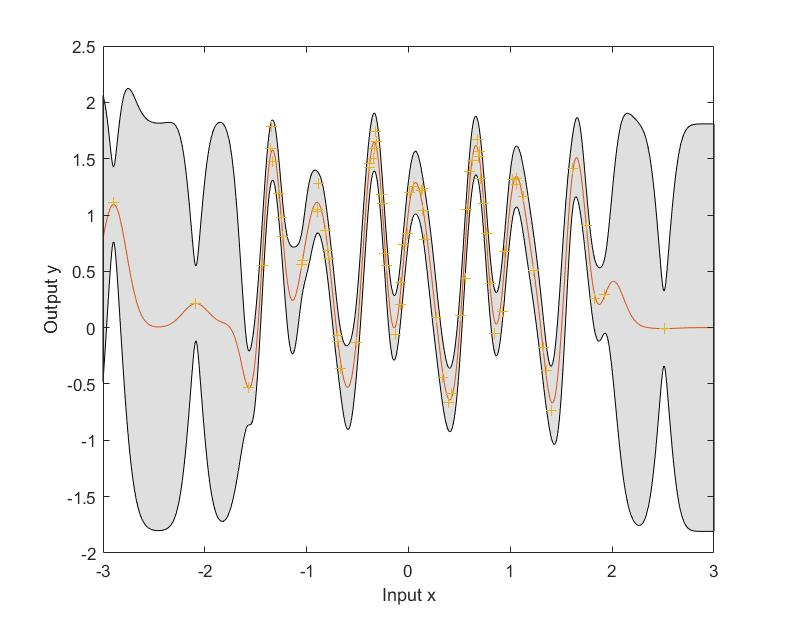
\includegraphics[width=0.3\paperwidth]{1a.jpg}\hspace{1cm}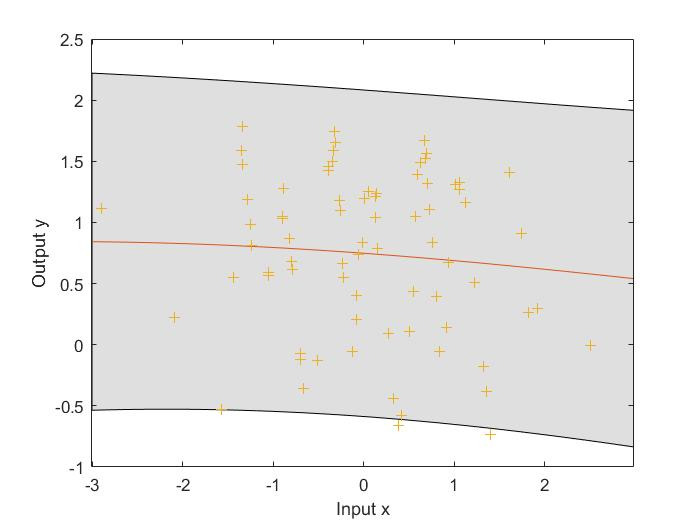
\includegraphics[width=0.3\paperwidth]{1b.jpg}
			\par\end{centering}
		\caption{ GP trained with SE covariance function with different local minima. 
			\newline  On the left, $\mathbf{\theta} = (l, \sigma, \sigma_n)= (0.128, 0.897, 0.118)  $ and $-\log(p(y|x, \mathbf{\theta})) = 11.9 $. 
			\newline  On the right, $\mathbf{\theta} = (l, \sigma, \sigma_n)= (8.042, 0.696, 0.663)  $ and $-\log(p(y|x, \mathbf{\theta})) = 78.2 $)
		 \label{fig:predictive_distributions} }
	\end{figure}

\newpage

\section{Local minima}

Our optimization function minimize a differentiable multivariate function using conjugate gradients. This method find the nearest local minimum to the initialization point. Therefore, by changing the initial hyper-parameters we expect to achieve other minima. For instance, by initializing \texttt(hyp.cov = [1, 0])  gives us another minimum for the marginal likelihood $\log(p(y|x,\theta)) = -78.2$. This corresponds to $\mathbf{\theta}= (8.042, 0.696, 0.663)$. From this, we expect our predictions to have error bars similar size.  

From the right side of Figure 1, we can see the our data is misinterpreted as noise. A large length scale implies an equivalent lower signal-to-noise ratio. 

Looking at the value of the marginal likelihoods, we can clearly see that the first model has a better value without even taking the exponential values. From this reasons, we can safely say that our first model is indeed the better one. 

\section{GP with a periodic covariance function}

In this section, we take a look at the same process implemented using a periodic covariance function.
This covariance has the following form
\begin{equation}
	k(x_i, x_j) = \sigma^2 \exp \left (-\frac{2\sin^2\left( \frac{\pi(x_i-x_j)}{p}\right)}{l^2}\right) + \delta_{ij} \sigma_{n}^2 
\end{equation}
where , $\sigma$, $l$, $\sigma_n$ have the same meanings as in section \ref{a}. The new hyper-parameter is the period of the functions $p$. 

\begin{figure}
	\begin{centering}
		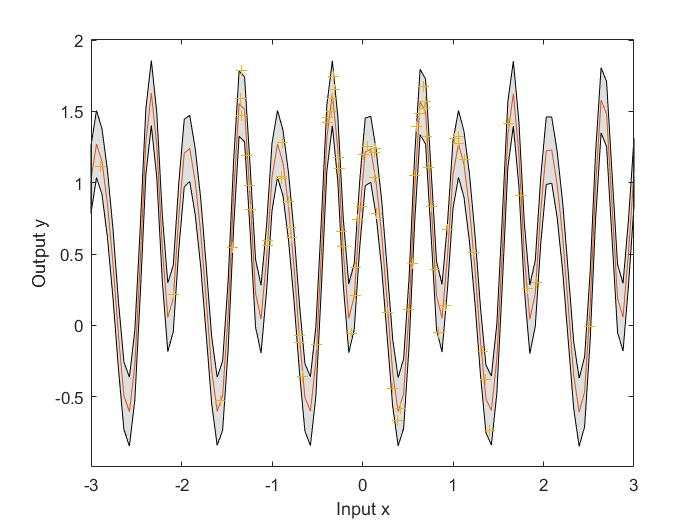
\includegraphics[width=0.5\paperwidth]{1c.jpg}
		\par\end{centering}
	\caption{Heat map plot of the the approximation of the model evidence obtained
		in the grid search.\label{fig:heat_map_plot} }
\end{figure}

We used the following initialization:

\begin{verbatim}
	covfunc = @covPeriodic; hyp.cov = [0, 0, 0]; hyp.lik = 1; %initialise hyperparameters
\end{verbatim}
and after following the same steps as before we get $\log p(y|x,\theta) = 35.2$ and $\theta = (l, p , \sigma, \sigma_n) =$\newline $  = (0.936, 0.999, 1.008, 0.110) $. We expect the error bars to be narrow as the signal-to-noise ratio is high($\sigma >> \sigma_n$). The lower bound for the error bars is $2\sigma_n$. Moreover, both the length scale and the period are approximately $1$. Therefore the signal should not change very much during one period and the functions should have a smoothly behaviour similar to sinusoidal. The periodicity of the model makes confident extrapolation making use of the highly dense data region repeatedly over the entire space.   

This periodic model not only fits the high number of data points in the central region, but also the isolated points. And on a first look we would choose this model although it is much restrictive. Indeed, if we have a look at the marginal likelihood has a better value than our first model.    
  
\section{Data generation}

For this task we will be using a combination of the SE covariation and periodic covariance.

\begin{equation}
	k(x_i, x_j) = \sigma^2 \exp\left( - \frac{(x_i - x_j)^2}{2 l_{SE}^2} \right)\exp \left (-\frac{2\sin^2\left( \frac{\pi(x_i-x_j)}{p}\right)}{l_{per}^2}\right)
\end{equation} 
 
By using the product of these two covariances we want to achieve a behaviour that is periodical in shape but its the shape is scaled by a mean component.

The hyper-parameters have the same meaning as in previous sections, but this time we have different length scales for periodicity and squared exponential. While $l_{per}$ looks at the smoothness inside one period, $l_{SE}$ acts on the smoothness of the mean modulator. As before, low $l_{per}$ corresponds to high oscillation inside one period and a high value corresponds to a smoother transition between the prediction. The value of $l_{SE}$ also acts as an indicator for the weighting of the models. A high value $l_{SE}$ result in the exponential tending to $1$. Thus, our covariance tends to be only periodical. Otherwise, for low-valued $l_{SE}$, our model will have high fluctuations outside the period and the SE covariance over-weights the periodic covariance. 

This implementation can be done using a new covariance matrix:

\begin{verbatim}
	K = feval( covfunc, hyp2.cov , xs);% find covariance matrix K
	K = K + 1e-6*eye(200); ;% make K positive definite ( stability )
	y = chol(K)'* randn( 200 , 1);% generate y from x
\end{verbatim}

The Cholesky decomposition works only on positive definite matrices. Therefore, we make sure that our matrix has positive eigenvalues by adding a diagonal matrix. Otherwise, due to finite precision of the computer the eigenvalues would be so small that they would be approximated to zero and the Cholesky method would fail.

\section{2-D fitting}

This time we will load the 2-D data from \texttt{cw1e.mat}. The only difference from previous sections is that our inputs for the \texttt{gp} function are 2-D. As we did before, we must first choose a covariance function for our model. This time with chose for our first model a Squared Exponential covariance function with Automatic Relevance Detemination (ARD) distance measure. This has the following form:

\begin{equation}
	k(x_i, x_j) = \sigma^2 \exp\left( - \frac{(x_i^{(1)} - x_j^{(1)})^2}{2 l_1^2}  - \frac{(x_i^{(2)} - x_j^{(2)})^2}{2 l_2^2}\right)
\end{equation}

As we can see the only difference from our first model is the, now, we have to hyper-parameters for the length scale $l_1$ and $l_2$, one for each dimension. The model predictions are shown in Figure 3 and the corresponding hyper-parameters are
$\theta = (l_1, l_2, \sigma, \sigma_{n}) = (1.5116, 1.2859, 1.1073, 0.1026)$ with a marginal likelihood of
$\log p(y|x,\theta) = 19.2$. As before, the length scales determine the smoothness in each direction. The small difference in magnitude shows a similar structure on both x1-axis and x2-axis.

\begin{figure}[h]
	\begin{centering}
		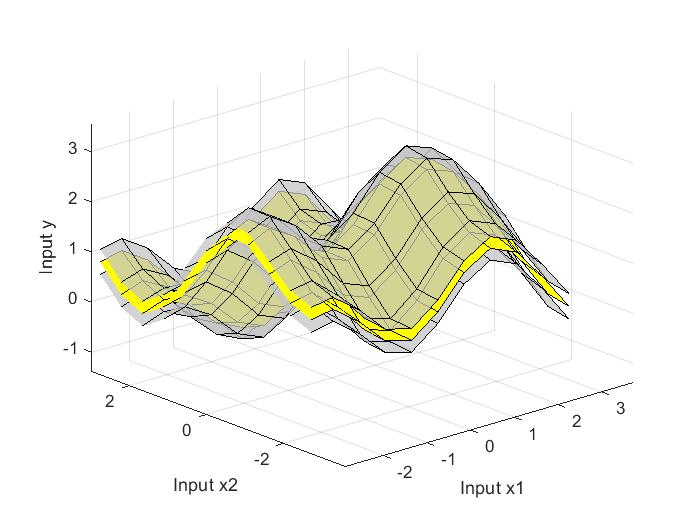
\includegraphics[width=0.3\paperwidth]{1e.jpg}\hspace{1cm}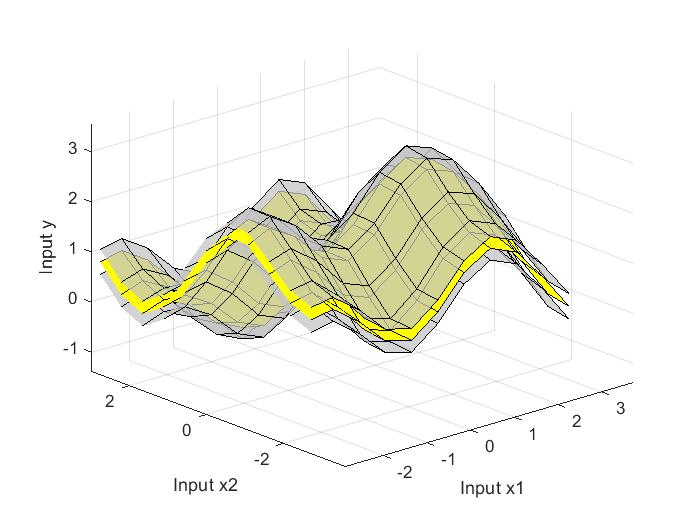
\includegraphics[width=0.3\paperwidth]{1e.jpg}
		\par\end{centering}
	\caption{ GP trained in 2-D with ARD. On the left, SEard. On the right, Sum of covariances
		\label{fig:predictive_distributions2} }
\end{figure}

Our second model wants to implement the sum of two ARD covariance functions as follows:

\begin{equation}
	k(x_i, x_j) = \sigma_1^2 \exp\left( - \frac{(x_i^{(1)} - x_j^{(1)})^2}{2 l_{11}^2}  - \frac{(x_i^{(2)} - x_j^{(2)})^2}{2 l_{12}^2}\right)  +\sigma_2^2 \exp\left( - \frac{(x_i^{(1)} - x_j^{(1)})^2}{2 l_{21}^2}  - \frac{(x_i^{(2)} - x_j^{(2)})^2}{2 l_{22}^2}\right)
\end{equation}

This model offers more flexibility as it account for different variances and dependencies on each input-axis. Moreover, its worst case scenario seems to be when one of the $\sigma$s collapses to zero and it ends up in the previous model. This flexible implementation guarantees a better marginal likelihood as long as we break the symmetry. If symmetry exits, our optimizer will see one $\sigma$ and one $l$ for each axis. Thus, this model should be almost always better, although it takes a bit more time to implement.  



\end{document}
